\section{Methodology}

\begin{figure}[h!]
  \centering 
    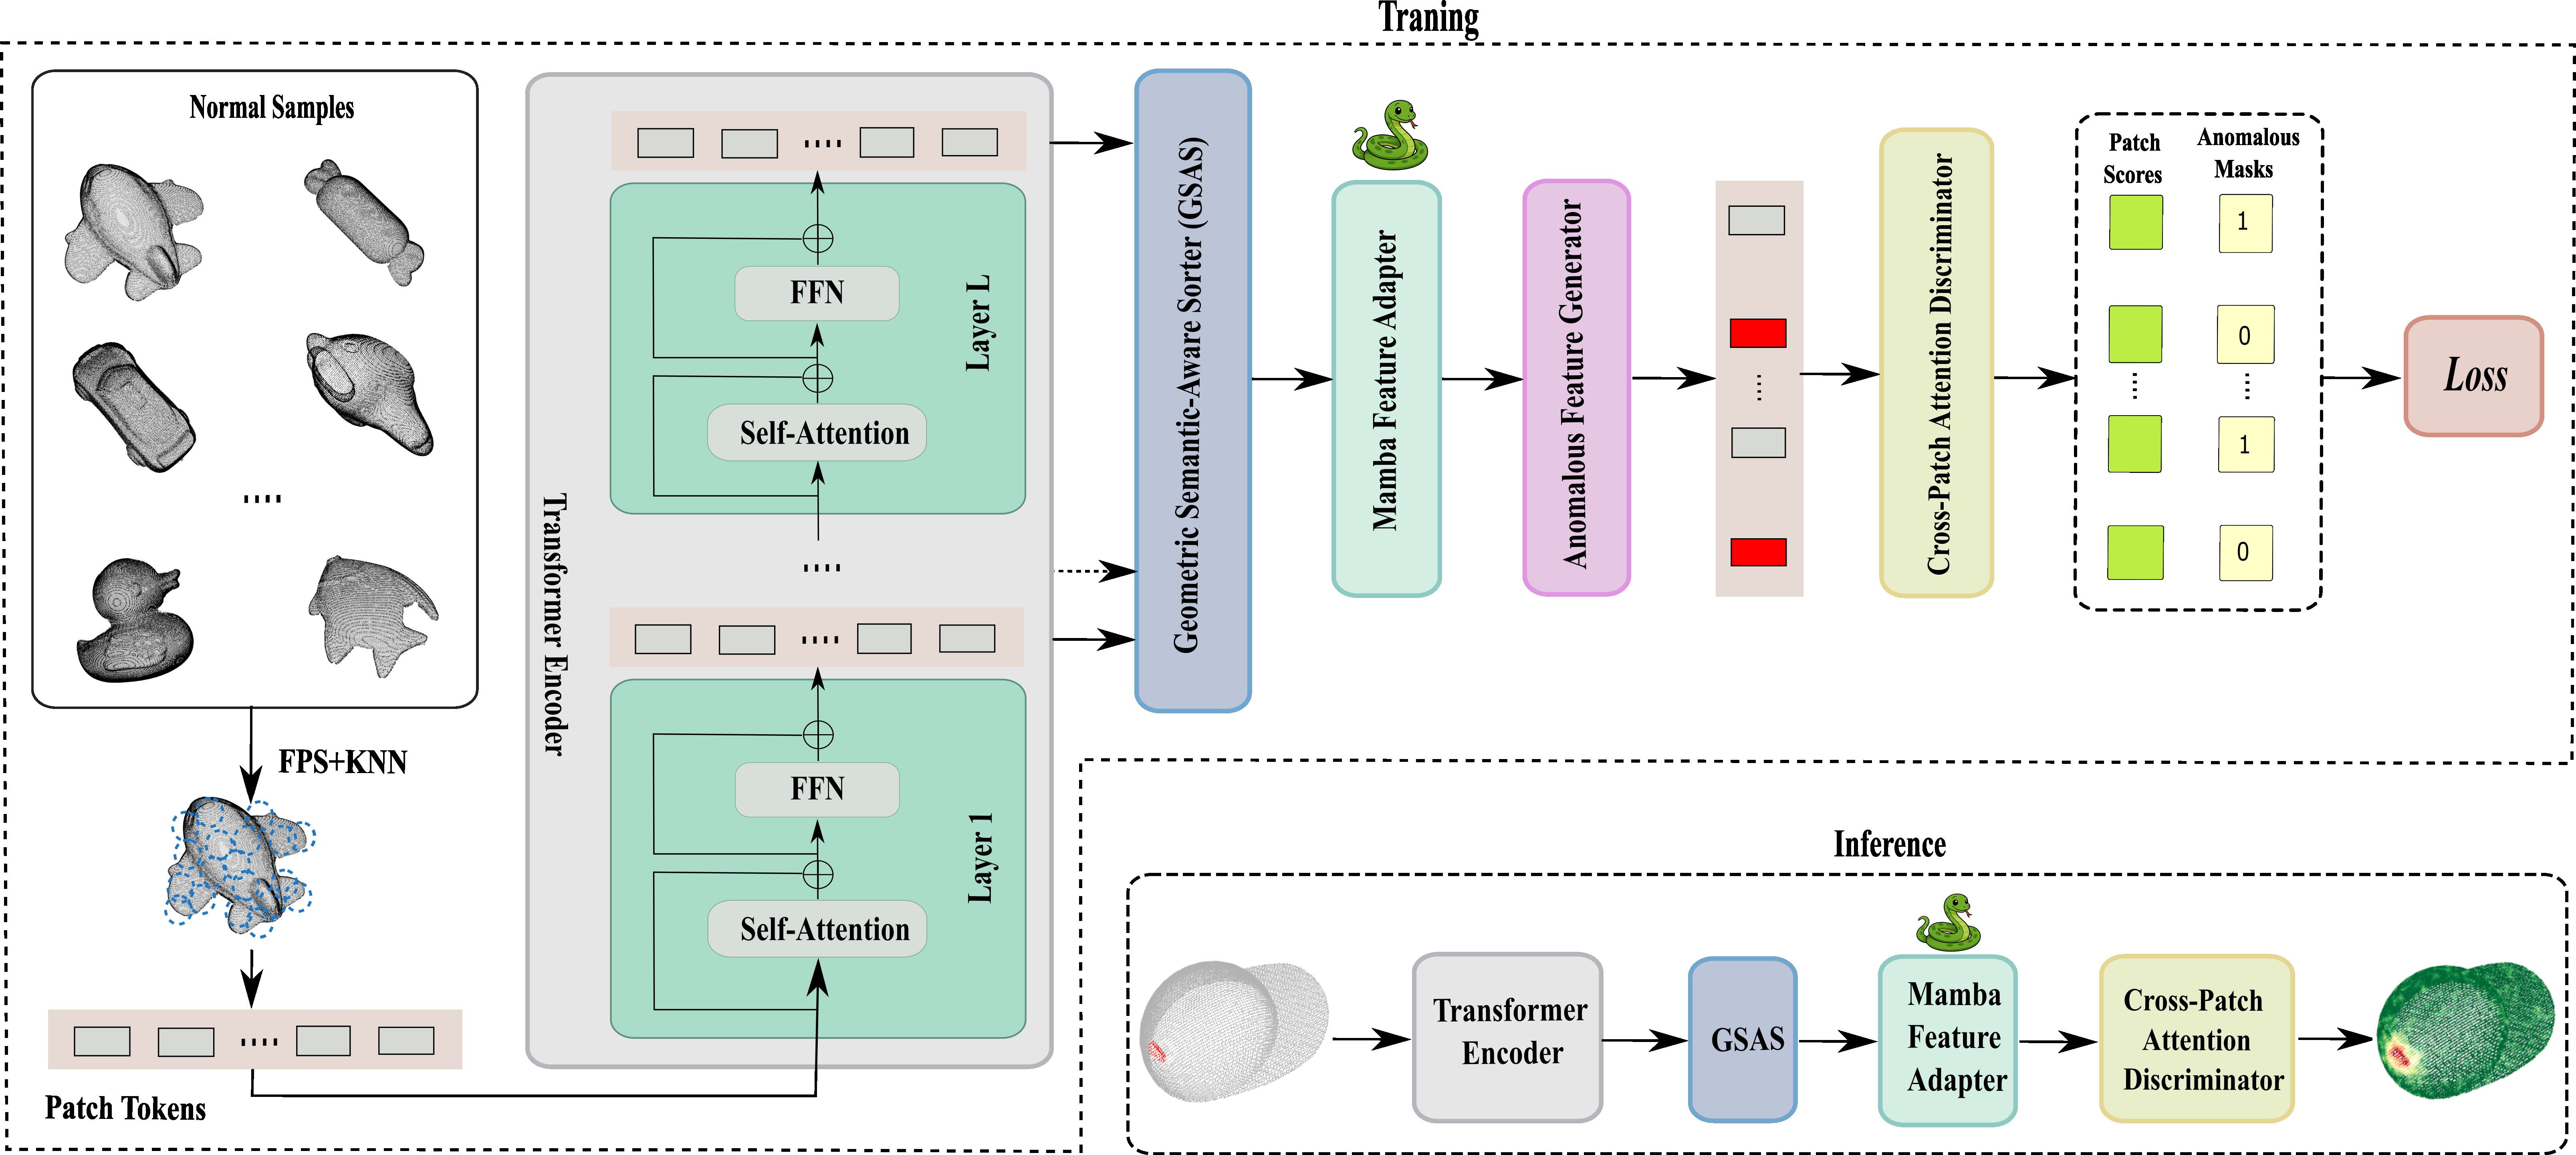
\includegraphics[width=0.98\linewidth]{figs/overview}
  \caption{Overview of the proposed 3D anomaly detection pipeline.}
  \label{fig:overview}
\end{figure}

We address efficient 3D anomaly detection that requires minimal task-specific training while preserving geometric structure and long-range contextual reasoning. As illustrated in Figure \ref{fig:overview}, given an input point cloud \(\mathcal{P} = \{\mathbf{p}_i \in \mathbb{R}^3\}_{i=1}^N\), the proposed pipeline leverages a frozen pre-trained point-cloud Transformer together with a compact set of lightweight adapters to generate spatially coherent and anomaly-sensitive representations. The backbone consists of \(L\) encoder layers, each producing \(M\) patch tokens of dimension \(D\); we denote the patch-token matrix and class token at layer \(i\) as \(\mathbf{T}_i \in \mathbb{R}^{M\times D}\) and \(c_i \in \mathbb{R}^{1\times D}\), respectively, and collect the hierarchical token set \(\mathbf{T} = \{\mathbf{T}_1, \dots, \mathbf{T}_L\}\) with a total of \(T = L \cdot M\) tokens. These unordered layer-wise tokens are transformed into a semantically ordered sequence \(\mathbf{T}_{\mathrm{ord}} \in \mathbb{R}^{T\times D}\), subsequently fused into enriched contextual features \(y_{1:T} \in \mathbb{R}^{T\times D}\), and finally scored by a lightweight attention-based discriminator for per-patch anomaly localization. The geometric semantic-aware sorter (GSAS) establishes a differentiable soft-permutation that orders the hierarchical tokens while preserving geometric locality and semantic consistency. The Mamba adapter, a linear-time state-space model, efficiently fuses the ordered sequence to yield context-enhanced features \(y_{1:T}\) that retain both local fidelity and global awareness. A selective anomaly generator operates during training to inject sparse feature-space perturbations, enabling effective supervision without real defect labels. The cross-patch discriminator then aggregates contextual cues through a compact attention mechanism to output patch-level anomaly logits, which are reprojected to points for precise localization. 

\subsection{Backbone}

Given an input point cloud \(\mathcal{P} = \{\mathbf{p}_i\in\mathbb{R}^3\}_{i=1}^N\), the backbone produces local patch embeddings and a hierarchical set of Transformer tokens that preserve patch identities across layers. We apply Farthest Point Sampling (FPS) to select \(M\) patch centers \(\{p_j\in\mathbb{R}^3\}_{j=1}^M\), where index \(j\) denotes a patch center, and for each center we collect a fixed-size neighborhood of \(K\) points via \(K\)-nearest neighbors (KNN). Each neighborhood is embedded by a lightweight PointNet encoder followed by a positional-encoding MLP to yield an initial patch embedding \(x_j^{(0)}\in\mathbb{R}^D\), for \(j=1,\dots,M\). The \(M\) initial embeddings are concatenated with a global class token \(c_0\in\mathbb{R}^{1\times D}\) to form the Transformer input \([c_0;\mathbf{T}_0]\), where \(\mathbf{T}_0=[x_1^{(0)};\dots;x_M^{(0)}]\in\mathbb{R}^{M\times D}\). These are passed to the frozen Point-MAE Transformer pretrained on ShapeNet~\cite{pang2022masked,chang2015shapenet}. Formally, the \(i\)-th Transformer block \(\ell_i(\cdot)\) computes
\begin{equation}
[c_i;\,\mathbf{T}_i] \;=\; \ell_i([c_{i-1};\,\mathbf{T}_{i-1}]), \qquad i=1,\dots,L,
\end{equation}
with \(\mathbf{T}_i=[t_{i,1};\dots;t_{i,M}]\in\mathbb{R}^{M\times D}\) and \(c_i\in\mathbb{R}^{1\times D}\). The spatial coordinates \(\{p_j\}\) remain associated with their patch index \(j\) and are reused at every Transformer layer; consequently token \(t_{i,j}\) at layer \(i\) corresponds to the same geometric patch center \(p_j\). The backbone therefore outputs the initial patch embeddings \(\{x_j^{(0)}\}_{j=1}^M\) with \(x_j^{(0)}\in\mathbb{R}^D\), the hierarchical tokens \(\{\mathbf{T}_i\}_{i=1}^L\) with \(\mathbf{T}_i\in\mathbb{R}^{M\times D}\), the sequence of class tokens \(\{c_i\}_{i=1}^L\) with \(c_i\in\mathbb{R}^{1\times D}\), and the retained patch centers \(\{p_j\}_{j=1}^M\in\mathbb{R}^3\). Optionally, these tokens may be viewed as a flattened set \(\mathbf{T}=\{\mathbf{T}_1,\dots,\mathbf{T}_L\}\) of \(T=L\cdot M\) tokens in \(\mathbb{R}^{T\times D}\).

\subsection{Geometric Semantic-Aware Sorter (GSAS)}
\label{sec:gsas}

\begin{figure}[h!]
  \centering 
    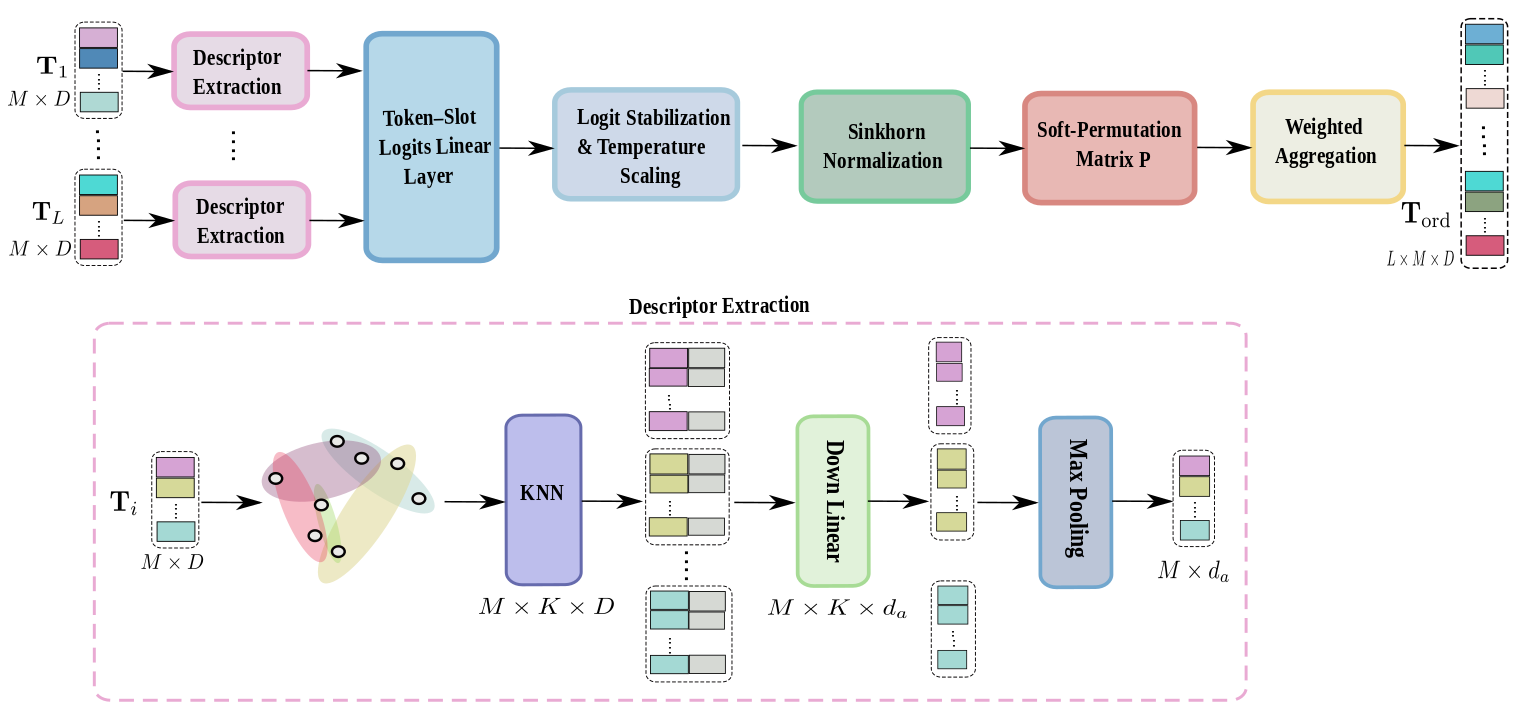
\includegraphics[width=0.98\linewidth]{figs/GSAS}
  \caption{Overview of geometric semantic-aware sorter (GSAS).}
  \label{fig:GSAS}
\end{figure}

Given input tokens \(X\in\mathbb{R}^{T\times D}\), where \(X\) denotes the flattened collection of all per-layer tokens \(t_{i,j}\) produced by the backbone (so that each \(\mathbf{T}_i=[t_{i,1};\dots;t_{i,M}]\in\mathbb{R}^{M\times D}\) and \(T=L\cdot M\)), and given the unique patch centers \(\{p_j\in\mathbb{R}^3\}_{j=1}^M\), GSAS produces a differentiable ordering of the \(T\) tokens that preserves local surface adjacency and semantic affinity. As illustrated in Figure ~\ref{fig:GSAS}, we first summarizes local geometry and same-layer semantics, then computes token-slot affinities, converts affinities to an approximately doubly-stochastic assignment, and finally aggregates tokens into ordered slots for downstream fusion.

We construct a kNN graph on the unique patch centers and denotes the neighbor set of patch \(j\) by \(\mathcal{N}_{\mathrm{patch}}(j)\subset\{1,\dots,M\}\). For a token \(t\) corresponding to \((i,j)\) with \(i=i(t)\) and \(j=j(t)\), GSAS computes a permutation-invariant local descriptor by aggregating features from the same Transformer layer \(i\) of neighboring patches:
\begin{equation}
u_{i,j} \;=\; \mathrm{MaxPool}\Big(\big\{\,W_{\downarrow}\,t_{i,u} + b_{\downarrow} \ \big|\ u\in\mathcal{N}_{\mathrm{patch}}(j)\big\}\Big)\in\mathbb{R}^{d_a},
\end{equation}
where \(W_{\downarrow}\in\mathbb{R}^{d_a\times D}\) and \(b_{\downarrow}\in\mathbb{R}^{d_a}\). The module collects these descriptors into \(E\in\mathbb{R}^{T\times d_a}\) by setting \(E_{t,:}=u_{i(t),j(t)}\). The descriptor \(E\) summarizes local geometry while preserving layer-specific semantics, and GSAS uses \(E\) to inform the affinity computation in the next step. We computes raw token-slot affinities from the descriptors:
\begin{equation}
\mathbf{G} \;=\; E\,W_{\uparrow} + \mathbf{1}\,b_{\uparrow}^\top \in\mathbb{R}^{T\times T},
\end{equation}
with \(W_{\uparrow}\in\mathbb{R}^{d_a\times T}\), \(b_{\uparrow}\in\mathbb{R}^T\), and \(\mathbf{1}\in\mathbb{R}^{T\times 1}\). The matrix \(\mathbf{G}\) encodes unnormalized affinities between tokens and ordered slots, and GSAS processes \(\mathbf{G}\) to produce a differentiable assignment that can be optimized end-to-end.

For numerical stability we subtract the column-wise maximum \(v\in\mathbb{R}^T\) with entries \(v_s=\max_t \mathbf{G}_{t,s}\), applies temperature scaling and exponentiation, and normalizes with the Sinkhorn operator:
\begin{equation}
\tilde{\mathbf{G}} \;=\; (\mathbf{G} - \mathbf{1}\,v^\top)/\tau,
\end{equation}
\begin{equation}
P \;=\; \mathrm{Sinkhorn}\big(\exp(\tilde{\mathbf{G}}),\,K_{\mathrm{sink}}\big)\in[0,1]^{T\times T},
\end{equation}
where \(\tau>0\) denotes the temperature and \(K_{\mathrm{sink}}\) the number of iterations. The soft-permutation \(P\) is approximately doubly-stochastic and differentiable, and GSAS uses \(P\) to aggregate token features into a semantically coherent ordered sequence. We aggregate tokens into ordered slots by weighted summation:
\begin{equation}
\mathbf{T}_{\mathrm{ord}} \;=\; P^\top X \in\mathbb{R}^{T\times D},
\end{equation}
\begin{equation}
\mathbf{T}_{\mathrm{ord}}[s,:]=\sum_{t=1}^T P_{t,s}\,X_t.
\end{equation}
The aggregation yields one feature vector per ordered slot while preserving differentiability so that gradients propagate to \(W_{\downarrow},b_{\downarrow},W_{\uparrow},b_{\uparrow}\). The ordered tokens \( \mathbf{T}_{\mathrm{ord}}\) therefore provide the contiguous, semantically coherent input required by the subsequent fusion module.

We include two auxiliary regularizers to prevent degenerate assignments and to encourage geometric locality. The column-wise entropy penalty discourages diffuse assignments into a given slot:
\begin{equation}
\mathcal{L}_{\mathrm{ent}} \;=\; \frac{1}{T}\sum_{s=1}^T H(P_{:,s}),\qquad
H(\pi)=-\sum_{t}\pi_t\log(\pi_t+\epsilon_{\mathrm{ent}}),
\end{equation}
with \(\epsilon_{\mathrm{ent}}>0\) for numerical stability. The entropy penalty directly biases the columns of \(P\) toward concentrated assignments and thus improves the quality of aggregation in Eq. for \(\mathbf{T}_{\mathrm{ord}}\). The locality penalty measures expected slot positions \(\mu_t\) and biases them to align with geometric affinities:
\begin{equation}
\mu_t \;=\; \sum_{s=1}^T \tilde s\,P_{t,s}\in[0,1],
\end{equation}
\begin{equation}
w_{t,u} \;=\; \exp\!\big(-\|p_{j(t)}-p_{j(u)}\|^2/\sigma_p^2\big),
\end{equation}
\begin{equation}
\mathcal{L}_{\mathrm{loc}} \;=\; \sum_{t=1}^T \frac{1}{\sum_{u=1}^T w_{t,u} + \epsilon_{\mathrm{norm}}}\sum_{u=1}^T w_{t,u}\,\big(\mu_t - \mu_u\big)^2,
\end{equation}
where \(\tilde s=(s-1)/\max(1,T-1)\), \(\sigma_p\) is a bandwidth parameter, and \(\epsilon_{\mathrm{norm}}>0\) stabilizes the normalization. The locality penalty directly influences \(\mu_t\) and thus biases the soft-permutation \(P\) to place geometrically adjacent tokens into nearby slots.

\subsubsection{Mamba Feature Adapter}

After GSAS produces the ordered token matrix $\mathbf{T}_{\mathrm{ord}}\in\mathbb{R}^{T\times D}$, let the row-wise sequence be
$$
x_{1:T},\qquad x_t=\mathbf{T}_{\mathrm{ord}}[t,:]\in\mathbb{R}^D,\quad t=1,\dots,T.
$$
The Mamba adapter is formulated as a state-space model that fuses long-range, layer-wise context along the GSAS-induced ordering. Let the latent dimension be $S$. The recurrence and output equations are defined as
\begin{equation}
h_t = A\,h_{t-1} + B\,x_t,\qquad h_0=\mathbf{0}\in\mathbb{R}^S,
\end{equation}
\begin{equation}
\tilde{q}_t = C\,h_t + D\,x_t \in\mathbb{R}^D,
\end{equation}
where
$$
A\in\mathbb{R}^{S\times S},\quad 
B\in\mathbb{R}^{S\times D},\quad 
C\in\mathbb{R}^{D\times S},\quad 
D\in\mathbb{R}^{D\times D}.
$$
The sequence of adapted outputs is collected as
$$
Q=[\tilde{q}_1,\dots,\tilde{q}_T]^\top\in\mathbb{R}^{T\times D},
$$
and, for consistency with the subsequent modules, $q_t\equiv\tilde{q}_t$.

The GSAS module determines the sequence order $x_{1:T}$, while the Mamba adapter performs contextual integration along this induced order without altering the token arrangement. The parameters $\{A,B,C,D\}$ are shared across all time steps, ensuring parameter efficiency and preserving the linear computational complexity with respect to sequence length $T$. Specifically, Mamba operates in $\mathcal{O}(T)$ time and requires $\mathcal{O}(S)$ additional memory per step, in contrast to the $\mathcal{O}(T^2)$ cost of full self-attention. The residual term $D\,x_t$ maintains per-token fidelity, while $C\,h_t$ introduces long-range contextual dependencies through the recurrent hidden state. The Mamba parameters are optimized jointly with the GSAS parameters, positional MLP, anomaly-scaling $\gamma$, and discriminator weights, whereas the Transformer backbone remains frozen.

\subsection{Anomalous Feature Generator}
Industrial defects in 3D point clouds are typically sparse, subtle, and spatially localized. To simulate such defects during training without requiring external anomaly examples, we introduce a lightweight, selective feature-space perturbation that synthesizes pseudo-anomalous tokens by injecting noise into a sparse subset of adapted token embeddings. Given output from Mamba feature adapter $Y$.

We sample an independent Bernoulli mask per token to determine corruption:
\begin{equation}
m_t \sim \mathrm{Bernoulli}(p),\qquad m_t\in\{0,1\},
\end{equation}
where \(p\in(0,1)\) controls expected corruption sparsity and is selected on validation (to reflect realistic, sparse defect rates we typically choose \(p\ll 0.5\) and tune it on held-out data). When \(m_t=1\) the token is corrupted by an additive isotropic Gaussian perturbation in the canonical token space:
\begin{equation}
\varepsilon_t \sim \mathcal{N}\big(0,\sigma^2 I_D\big),
\end{equation}
where \(\sigma>0\) controls perturbation scale (we validate \(\sigma\); a practical value is \(\sigma=0.1\)). The pseudo-anomalous token is defined as
\begin{equation}
\tilde{q}_t \;=\; q_t + \gamma\, m_t\, \varepsilon_t,
\end{equation}
where \(\gamma\ge 0\) is a learnable scalar that adaptively rescales the injected perturbation (initialized to a small positive value). When \(m_t=0\) we have \(\tilde{q}_t=q_t\). This corruption mechanism is applied only during training; at inference time the generator is disabled (\(m_t\equiv 0\)) and all tokens remain clean.

The selective (sparse) corruption contrasts with indiscriminate global noise: by corrupting a small fraction of slots we emulate localized defects while preserving the normal manifold for the majority of features. Because sparse corruption can induce class imbalance, we (i) recommend validating \(p\) on held-out data and (ii) mitigate imbalance via weighted loss or controlled sampling (details in the training section).

\subsection{Cross-Patch Attention Discriminator}
Detecting defects often requires contextual comparison across patches. We therefore employ a lightweight attention-based discriminator that jointly processes all patch slots and outputs a scalar logit per slot. To preserve spatial information and to generalize across varying patch arrangements, positional embeddings are derived from patch center coordinates rather than learned per-slot indices. Let \(p_t\in\mathbb{R}^3\) denote the patch center associated with slot \(t\); the positional embedding is computed by a small coordinate MLP:
\begin{equation}
e_t \;=\; \mathrm{PE\text{-}MLP}(p_t) \in\mathbb{R}^D.
\end{equation}

During training we construct a single mixed input sequence for the discriminator in which corrupted tokens replace clean tokens in-place. The discriminator input for slot \(t\) is therefore
\begin{equation}
\hat{q}_t \;=\; \big(m_t\,\tilde{q}_t + (1-m_t)\,q_t\big) + e_t \;=\; q_t + m_t(\gamma\varepsilon_t) + e_t,
\end{equation}
and the supervision label is \(y_t=m_t\). Inference uses the same pipeline but with \(m_t\equiv 0\) so that \(\hat{q}_t=q_t+e_t\).

Let \(H\) denote the number of attention heads and \(d_{\mathrm{head}}=D/H\) the per-head dimension; in practice we choose \(D\) divisible by \(H\) or insert a thin linear projection to meet this constraint. The discriminator applies a single multi-head self-attention layer followed by a compact shared MLP head that maps each token to a scalar logit:
\begin{align}
Z \; &=\; \mathrm{MHA}(\{\hat{q}_t\}_{t=1}^T)\in\mathbb{R}^{T\times D},\\
s_t \; &=\; \mathrm{MLP}_{\mathrm{head}}(Z_t)\in\mathbb{R}.
\end{align}
Here \(\mathrm{MHA}(\cdot)\) denotes standard multi-head self-attention with appropriate query/key/value projections, scaled dot-product attention, residual connections, dropout and layer normalization; \(\mathrm{MLP}_{\mathrm{head}}\) is a two-layer feedforward network (one hidden layer) shared across slots and producing a scalar logit. Layer normalization and dropout are included to stabilize training. Because the discriminator processes all tokens jointly, each output \(s_t\) reflects both local evidence and global context, improving sensitivity to structured or context-dependent defects compared to independent per-slot scoring.

At test time the discriminator receives only clean tokens \(\{q_t\}\) augmented with positional embeddings \(e_t\) and outputs per-slot logits \(s_t\). These per-slot scores are reprojected to the original point cloud by assigning each point the maximal score of the patches that contain it (see Inference section).

\subsection{Loss Function and Training}
\label{sec:loss}

We jointly optimize the trainable components (GSAS parameters, Mamba adapter parameters, positional-embedding MLP, the anomaly-scaling \(\gamma\), and discriminator parameters) using a patch-wise binary classification objective. Let \(\Theta\) denote the set of all trainable parameters. For a training batch we accumulate \(P\) supervised token slots (summed across batch and sequence). We use a numerically-stable logits-based binary cross-entropy implemented as BCE-with-logits. The per-slot logits-based loss (stable form) is:
\begin{equation}
\ell_{\mathrm{BCElogits}}(s,y) \;=\; \max(s,0) - s\,y + \log\big(1+\exp(-|s|)\big),
\end{equation}
and the unweighted batch loss is \(\mathcal{L}_{\mathrm{BCE}}=\frac{1}{P}\sum_{t=1}^P \ell_{\mathrm{BCElogits}}(s_t,y_t)\). To mitigate class imbalance when corruption is sparse we optionally use a positive-class weighting factor \(w_+>0\) (e.g., \(w_+=(1-p)/p\) or a value tuned on validation) via the standard \texttt{pos\_weight} mechanism of BCE-with-logits; this multiplies the contribution of positive (corrupted) examples.

We complement \(\mathcal{L}_{\mathrm{BCE}}\) with the GSAS regularizers \(\mathcal{L}_{\mathrm{ent}}\) and \(\mathcal{L}_{\mathrm{loc}}\) (defined in Sec.~\ref{sec:gsas}) to discourage diffuse soft assignments and to encourage geometric locality in the induced ordering. The total objective is therefore
\begin{equation}
\mathcal{L} \;=\; \mathcal{L}_{\mathrm{BCE}} \;+\; \alpha_{\mathrm{ent}}\,\mathcal{L}_{\mathrm{ent}} \;+\; \alpha_{\mathrm{loc}}\,\mathcal{L}_{\mathrm{loc}},
\end{equation}
where \(\alpha_{\mathrm{ent}},\alpha_{\mathrm{loc}}\ge 0\) are small weighting coefficients selected on validation. Weight decay and parameter regularization are handled via AdamW's decoupled weight-decay (i.e., we pass the weight-decay hyperparameter to the optimizer rather than applying an explicit \(\ell_2\) penalty inside \(\mathcal{L}\)). In practice we use AdamW with initial learning rate \(10^{-4}\), cosine annealing over 100 epochs, batch size 8, and gradient clipping (norm limit 1). Standard 3D augmentations (random yaw, point jittering, scaling) are applied prior to patch extraction.

During training the discriminator receives a single mixed set of tokens (some corrupted in-place, others clean) and predicts per-slot logits \(s_t\) with labels \(y_t=m_t\). We do not present both clean and corrupted duplicates of the same cloud in the same forward pass; the single-stream mixed-input design matches inference-time behavior and simplifies batching.

\subsection{Inference and Scoring Function}

At inference the Anomalous Feature Generator is disabled (i.e., \(m_t\equiv 0\) and \(\tilde{q}_t=q_t\)). The deterministic pipeline is: extract patches and patch centers \(\{p_j\}\) (shared across layers), compute Transformer tokens and apply GSAS to obtain an ordered sequence, run the Mamba adapter to obtain adapted tokens \(q_t\), compute positional embeddings \(e_t=\mathrm{PE\text{-}MLP}(p_t)\), and evaluate the trained discriminator to obtain logits \(s_t\). Optionally convert logits to probabilistic intensities via \(\sigma(s_t)\).

To reproject per-slot scores to the original point cloud, assign each point \(\mathbf{x}\) the maximum logit among patches that contain it:
\begin{equation}
s(\mathbf{x}) \;=\; \max_{t:\,\mathbf{x}\in\mathcal{P}_t} s_t,
\end{equation}
where \(\mathcal{P}_t\) denotes the set of input points belonging to patch \(t\) (from the KNN used at patch extraction). A 3D median filter or voxel-grid median aggregation may be applied to the resulting heatmap for spatial smoothing; the filter kernel size or voxel resolution is selected on validation. For segmentation the heatmap is thresholded at \(\tau_{\mathrm{seg}}\) (chosen on validation), and for global anomaly detection we compute the cloud score
\begin{equation}
s_{\mathrm{cloud}} \;=\; \max_{t} s_t,
\end{equation}
declaring the cloud anomalous if \(s_{\mathrm{cloud}}>\tau_{\mathrm{pc}}\).

Implementation notes: we maintain a single canonical token dimension \(D\) throughout; positional embeddings are coordinate-derived via \(\mathrm{PE\text{-}MLP}\) to generalize across patch arrangements; the discriminator head count \(H\) is chosen so \(D\) is divisible by \(H\) (or a thin projection is applied); and hyperparameters \(p,\sigma,\gamma,\alpha_{\mathrm{ent}},\alpha_{\mathrm{loc}},w_+\) and median-filter settings are selected on validation and reported in the experimental section.
